%%%% ijcai11.tex

\typeout{IJCAI-11 Instructions for Authors}

% These are the instructions for authors for IJCAI-11.
% They are the same as the ones for IJCAI-07 with superficical wording
%   changes only.

\documentclass{article}
% The file ijcai11.sty is the style file for IJCAI-11 (same as ijcai07.sty).
\usepackage{ijcai11}

% Use the postscript times font!
\usepackage{times}

\usepackage{graphicx}
\usepackage{url}
\usepackage{bbding}
\usepackage{subfig}
\usepackage{listings}
\usepackage{pageslts}
% the following package is optional:
%\usepackage{latexsym} 

% Following comment is from ijcai97-submit.tex:
% The preparation of these files was supported by Schlumberger Palo Alto
% Research, AT\&T Bell Laboratories, and Morgan Kaufmann Publishers.
% Shirley Jowell, of Morgan Kaufmann Publishers, and Peter F.
% Patel-Schneider, of AT\&T Bell Laboratories collaborated on their
% preparation.

% These instructions can be modified and used in other conferences as long
% as credit to the authors and supporting agencies is retained, this notice
% is not changed, and further modification or reuse is not restricted.
% Neither Shirley Jowell nor Peter F. Patel-Schneider can be listed as
% contacts for providing assistance without their prior permission.

% To use for other conferences, change references to files and the
% conference appropriate and use other authors, contacts, publishers, and
% organizations.
% Also change the deadline and address for returning papers and the length and
% page charge instructions.
% Put where the files are available in the appropriate places.


\title{Model Transformation and Web Interface for Verifying BPMN Processes}
\author{Ajay Krishna Muroor Nadumane \\ 
Universit{\'e} Grenoble Alpes - Grenoble INP - Inria\\
Grenoble, France \\
muroorna@e.ujf-grenoble.fr \\
\\
Supervised by: Gwen Sala{\"{u}}n, Universit{\'e} Grenoble Alpes - Inria - LIG, France} % Mosig student

\begin{document}
\pagestyle{plain}
\setcounter{page}{1}
\pagenumbering{arabic}

\maketitle

{% Mosig student
  {\hbox to0pt{\vbox{\baselineskip=10dd\hrule\hbox
to\hsize{\vrule\kern3pt\vbox{\kern3pt
\hbox{{\small I understand what plagiarism entails and I declare that this report }}
\hbox{{\small is my own, original work.}} 
\hbox{{\small Name, date and signature: \hspace{20mm} Ajay Muroor, 14/6/16}}
\kern3pt
}\hfil%\kern3pt
\vrule
}\hrule}
}}
}


\begin{abstract}
Business process evolve over time and there are not many tools available to measure the quality of evolved process. VBPMN framework is aimed at formal verification of BPMN models which can be a measure of quality. This paper describes the model-to-model transformation of BPMN models to an intermediate format and integration of components in the context of VBPMN framework. The intermediate format serves as a link between XML based BPMN models and formal verification tools. Various components of the framework are integrated through an interface that allows process designers to compare BPMN 2.0 models. The interface abstracts the complex interactions with verification tools, making it appealing for adoption in the broader BPM community.
\end{abstract}


\section{Introduction}

A business process consists of set of tasks and activities, which may involve various participants, to accomplish a specific organizational 
goal \cite{Appian:BP}. Gartner defines Business Process Management (BPM) as ``\textit{the discipline that uses various methods to discover, model, 
analyze, measure, improve, and optimize business processes}'' \cite{Gartner:BPM}. 
\textit{Business Process Model and Notation} (BPMN) provides a standard graphical notation to represent the business processes. It can 
be used to manage the processes within the organization and also to share the processes across organizations. BPMN 2.0 is the \textit{Object Management Group} (OMG) standard \cite{omg2011bpmn} that is currently in existence for modelling of business processes. 

As the businesses grow, their processes evolve, they find ways to optimize their processes or refactor the existing processes. Organizations can benefit if they could measure the quality of the new process in comparison to the previous process. Comparison using formal verification tools can provide useful insights on how to optimize the process further or help identifying the shortcomings of the new process. Business process modelling tools like Activiti, Bonita BPM and Obeo BPM Designer do not offer much support in controlling the evolution of processes - they do not provide ways to check if the evolution is correct. \textit{Verification of BPMN} (VBPMN) \cite{Salaun:Malaga} is a framework that is being developed at Inria to support such verifications. The goal of VBPMN is formal modelling of business processes and automated analysis of such processes using formal verification tools. An overview of the framework is shown in Figure \ref{fig:vbpmn}.

\begin{figure}[ht]
\center
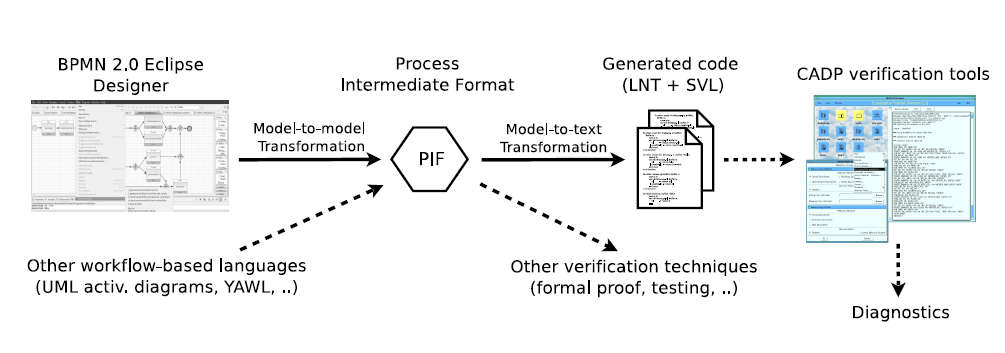
\includegraphics[width=1.0\linewidth]{Fig1.png}
\caption{VBPMN Framework}
\label{fig:vbpmn}
\end{figure}
VBPMN framework does process verification using model checking techniques. It is achieved by defining a model transformation that translates a BPMN model into a formal model. This formal model is used for analysis and to check the correctness of evolutions. As shown in Figure \ref{fig:vbpmn}, model transformation relies on an intermediate XML scheme called \textit{Process Intermediate Format} (PIF). PIF is a representation of elements of interest from the models. As the work is also planned to support different workflow models like UML and \textit{Yet Another Workflow Language} (YAWL), PIF serves as a generic, common template for building a workflow model. 

The objectives of this internship were to study the existing modelling tools available in the market, later develop an automated transformation of BPMN models generated using these tools to PIF. Beyond automation, the goal was to integrate the transformation component to existing backend analysis features and to provide an interface for process designers to leverage the framework capabilities. Finally, we had to validate this approach through several real world examples. 

The paper is further organized into three more sections, next section details the existing processes and related work. Section 3 contains the information about front-end, model-to-model transformation and integration with 
VBPMN framework. In section 4, performance of transformation component is described from the perspective of validating our approach. The last section focuses on concluding remarks and intended future work.

\section{Background}
\subsection{Related Work}
A considerable amount of work has been previously done on formal modelling, verification and analysis of business processes. In the earlier work \cite{Choreo:Ref}, had proposed transformation from BPMN to \textit{LOTOS New Technology} (LNT) \cite{LNT:Ref} for checking realizability of  BPMN choreographies using state machine patterns. The current work provides not just a platform for formal analysis and verification of a single process but also an interface to compare two processes from the perspective of evolution. In other related work, \cite{Lam:Ref}, equivalence behaviour is approached from theoretical point of view. \cite{Boud:Ref} presents evolution from a migration perspective. VBPMN takes a different approach, building on a comparison model with various choices for model matching.

\subsection{Existing Infrastructure}
Existing BPM modelling tools like Activiti and Bonita BPM generate BPMN 2.0 compliant models. The process models are internally represented in a XML scheme conforming to BPMN 2.0 specification \cite{omg2011bpmn}. 

As shown in Figure \ref{fig:vbpmn}, BPMN 2.0 XML models undergo transformation conforming to the PIF scheme. Once the PIF transformation is complete, they undergo model-to-text transformation to generate LNT encodings and \textit{Script Verification Language} (SVL) \cite{SVL:Ref} files. LNT is a formal specification language used for specifying and verifying concurrent systems. LNT is extensively used for specifying and verifying concurrent systems using \textit {Construction and Analysis of Distributed Processes} (CADP) \cite{CADP:Ref}. SVL behaves as a tool-independent coordination language on top of CADP. SVL offers high-level operators for generation, parallel composition, minimization, label hiding, label renaming, abstraction, comparison and model-checking of \textit{Labelled Transition Systems}(LTSs). These generated files are given as an input to CADP verification toolbox to identify behavioral equivalence among models. In case of failure to satisfy the equivalence condition, a counterexample is generated so that the model under consideration can be reviewed. In the earlier work \cite{VBPMN:Ref}, PIF has been formalized and work on model-to-text transformation has been accomplished. This paper primarily covers the work on model-to-model transformation of BPMN 2.0 models generated using popular modelling tools into PIF and integration of framework components. 

In the back-end model-text-transformation, the modes of comparison has already been defined \cite{VBPMN:Ref} to evaluate an evolution of a process. \textit{Conservative comparison} is the strictest of all available comparisons and it matches all the observable behaviors using the notion of strong equivalence \cite{Milner:Book}. \textit{Inclusive comparison} is more flexible, which in turn it allows extension of process models. It allows the extended model to match as long as existing behavior is unchanged. \textit{Exclusive comparison} supports refactoring involving reduction. Suppose, a process needs to be refined so that it involves only a part of existing activities, exclusive comparison ensures that the new behavior is identical as if it has been extracted from old process. The inclusive and exclusive comparisons are complementary modes in checking evolution. The aforementioned comparisons take the whole process into account, but selective comparison is also supported. \textit{Selective comparison} allows to match only the behaviors of tasks under consideration. It is done by hiding the tasks that are not under consideration in the backend. Renaming is another aspect supported by the framework. As the process evolves, it is possible that the elements get renamed. Backend uses relabeling relation \cite{VBPMN:Ref} to perform equivalence checking on evolutions with renaming. Another feature supported is \textit{property-aware comparison} where evolution is checked against properties of interest like deadlock freedom. Properties to be verified are specified using temporal logic. 

\section{Approach and Work}
VBPMN framework aims to take the power of CADP, a state-of-art verification toolbox to business process developers by providing an interface that abstracts complex interactions. To make it possible, we propose a user interface and a generic BPMN 2.0 model to PIF model transformation engine within the purview of VBPMN framework. 

\subsection{BPMN Elements and Transformation}
Transformation component of the VBPMN framework is responsible for transforming the BPMN models into PIF representation. The transformation process is kept as generic as possible to support other workflow models in the future. 

PIF is an XML based generic scheme for workflow models. It is designed to utilize several formal verification tools in the back-end. Since PIF is generic, the elements of the PIF do not directly map to the BPMN elements. The core element of PIF is Workflow Node which captures different elements in a workflow model along with its incoming and outgoing flows. In the current scope of work, we have considered only a subset of BPMN elements to be represented in PIF. Figure \ref{fig:elements} shows the BPMN elements considered during transformation.

\begin{figure}[h]
\center
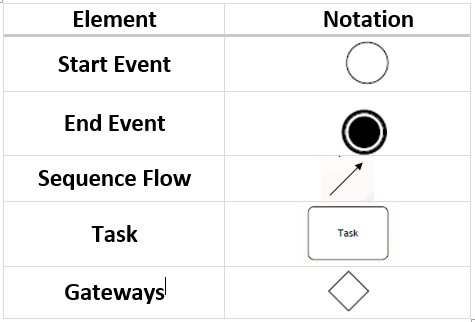
\includegraphics[scale =0.6]{Table1.png}
\caption{Elements considered for transformation}
\label{fig:elements}
\end{figure}

Transformation is straightforward for \textit{start}, \textit{end} events and \textit{tasks} as these elements can be directly mapped in the PIF XML representation. 
BPMN allows flexibility in representing sequence flows. It is optional to declare the incoming and outgoing flows of an element within the element. So during transformation, if the flows are not defined within the element we capture the element’s incoming and outgoing flows from the \textit{sequence flow} element of the BPMN model.

BPMN gateways are of much interest from the verification point of view. There are five different gateways in BPMN as listed in Figure \ref{fig:gateways}.

\begin{figure}[h]
\center
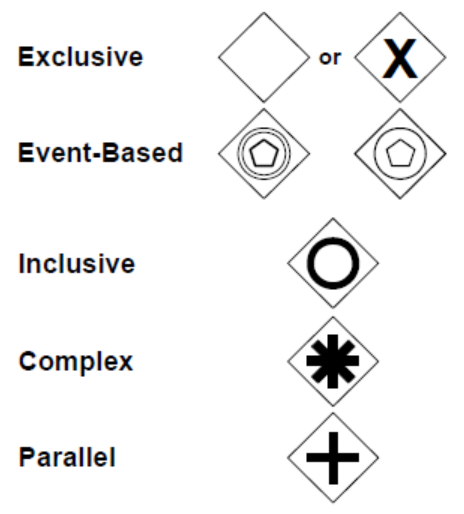
\includegraphics[scale =0.8]{Gateway.png}
\caption{BPMN Gateways}
\label{fig:gateways}
\end{figure}

An \textit{Exclusive} gateway represents a unique decision path out of a number of available paths. It can be used to create alternative paths within the process flow. An \textit{Inclusive} gateway, represents the possibility of taking one, multiple or all of the available paths after evaluating all the condition expressions. \textit{Parallel} gateways can be used to create unconditional parallel flows. The path in an Event based gateway is triggered by an event. The decision is made based on the data that is not visible to the process. The gateway behavior can be classified as two patterns – \textit{split} pattern and \textit{merge} pattern as shown in Figure \ref{fig:splitmerge}

\begin{figure}[ht]
\center
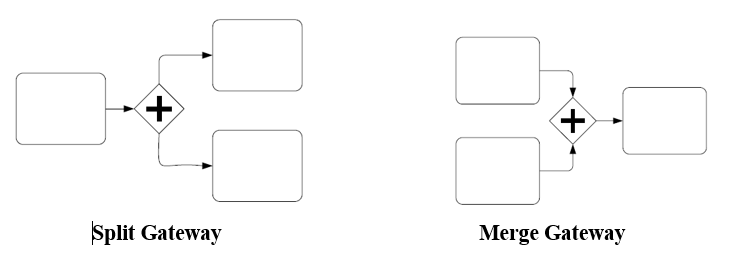
\includegraphics[scale =0.6]{MergeSplit.png}
\caption{Gateway Patterns}
\label{fig:splitmerge}
\end{figure}

Diverging flows follow the split pattern and converging flows follow the merge pattern. An exclusive gateway in merge pattern is used to combine alternative paths and also to construct looping behavior. Inclusive gateway in merge pattern can be used to combine a set of alternative and parallel paths. Merging parallel gateways wait until all the incoming flows are evaluated before triggering the execution of outgoing flow. Complex gateways, which are used to model complex synchronization behavior is not considered for the current iteration of the Transformation component.
 
PIF XML scheme does not provide direct mapping for BPMN gateways. Instead, during the transformation, BPMN gateways are mapped to their logical equivalent elements in PIF. The BPMN gateways and their equivalent PIF gateways are listed in Table \ref{tab:gways}

\begin{table}[ht]
\centering
\begin{tabular}{|l|l|}
\hline
BPMN Gateway & PIF Gateway \\
\hline \hline
Exclusive & XOR \\
\hline
Inclusive & OR \\
\hline
Parallel & AND \\
\hline
Event Based & XOR \\
\hline
\end{tabular}
\caption{BPMN and PIF Gateways}
\label{tab:gways}
\end{table}

Each gateway in PIF is identified as split or join gateway. If a gateway has more incoming flows than outgoing flows, it is treated as a merge gateway, otherwise it is treated as split gateway during transformation.

The Transformation component does a sequential line by line parsing of BPMN elements, each element is parsed and transformed into PIF element. It assumes that the BPMN model is valid and BPMN 2.0 compliant. The BPMN elements that are not listed in Figure \ref{fig:elements} are not handled during parsing and they will not appear in the PIF representation of the model. As PIF is intended to support multiple workflow models, it is of little benefit, if we are to incorporate the whole expressive nature of BPMN elements, especially the ones which are quite specific to BPMN. The high level process flow of the transformation is represented in Figure \ref{fig:transformation}.

\begin{figure}[ht]
\center
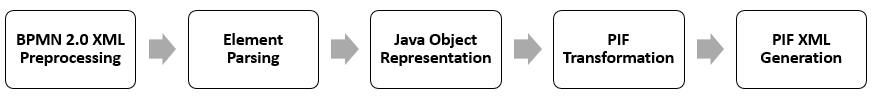
\includegraphics[scale =0.58]{Transformation.png}
\caption{Transformation Sequence}
\label{fig:transformation}
\end{figure}

During the initial stage of transformation, a preprocessing of BPMN XML model is done to strip off unnecessary information. Parsing step parses the entire document but considers only the elements of interest. These elements are mapped into PIF elements during the transformation stage. The PIF representation corresponding to the model is generated as an XML file, validated against the PIF \textit{XML Scheme Document} (XSD) and will be used in the subsequent processes. 

\subparagraph{User Interface}
The proposed interface is designed to support all of those comparisons defined in the previous section. The source for comparison are BPMN 2.0 XML files corresponding to the original and evolved model. Along with the results of comparison, the interface provides an option to view the counter example in case of a mismatch for the chosen mode of comparison. In the backend, the user interactions invoke transformation component and connect to backend python scripts to perform verification and analysis.

\subsection{Component Architecture}

VBPMN framework is designed to reach a large community of BPM users who need not be bogged down by the complexities of verification tools. So usability is an important factor in designing framework components. The components provide simple interaction mechanisms yet leverage the power of state of art verification tools. The technology stack is shown in Figure \ref{fig:techstack}.

\begin{figure}[ht]
\center
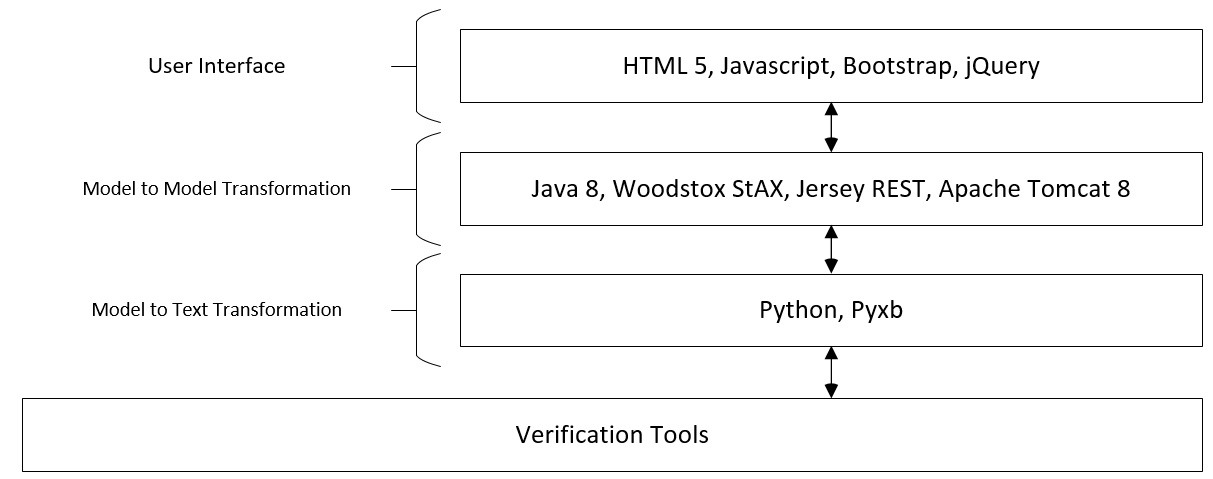
\includegraphics[scale =0.4]{TechStack.png}
\caption{VBPMN Technology Stack}
\label{fig:techstack}
\end{figure}

The transformation component is based on Java. It uses \textit{Streaming API for XML} (StAX) \cite{Stax:Ref} readers for parsing of BPMN models. Once the elements are parsed, they are stored as intermediate Java objects before being transformed into PIF XML document. Intermediate Java representation closely resembles the PIF in object world. So in future, if any other workflow model (for example, UML) needs to be integrated into the framework, it only needs to be transformed into object representation and it can re-use the existing object to PIF transformation components. 

\begin{figure}[ht]
\center
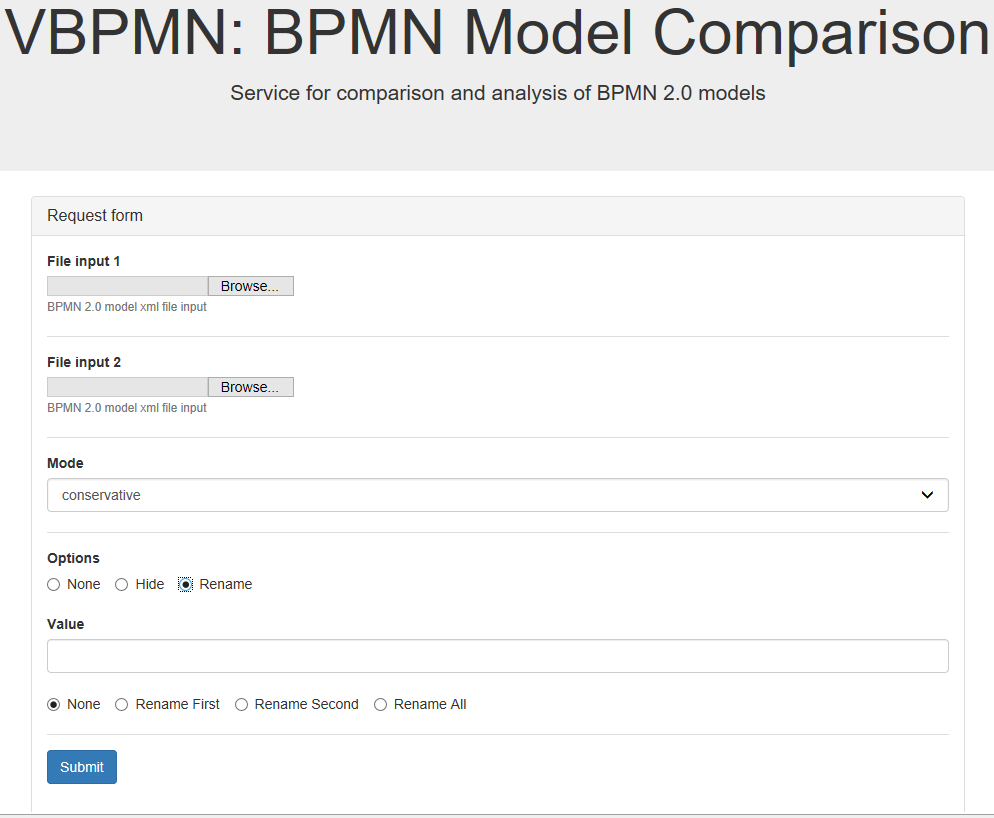
\includegraphics[scale =0.4]{UI.png}
\caption{User Interface}
\label{fig:ui}
\end{figure}

The transformation component is also integrated with VBPMN Python scripts. These scripts perform PIF to LNT transformation and interact with CADP for verification and analysis. The scripts are invoked from Java through its APIs, which has similar effect to invoking from the system terminal. All the comparison options are built within the transformation component and exposed as a \textit{Representational State Transfer} (REST) API. The idea behind developing a REST API is that it offers a flexible pluggable interface which is not tightly coupled to the user interface. It also allows us to add more APIs in the future and cater more modelling tools without affecting the existing interfaces.
 
The BPMN model comparison user interface is built using HTML5 and JavaScript. It invokes the REST APIs to render content to the user. Various comparison options are presented to the user through a web form as shown in Figure \ref{fig:ui}. Unlike an Eclipse plugin, a web interface can be independently used without having the need for Eclipse dependencies. Web interface can serve multiple screen forms too. 

All these components are packaged and hosted on an Apache Tomcat server. Hosting allows to wrap all the components  and their dependencies and provide a single window for interaction.

\section{Validation}
The experiments to validate framework performance and integration where conducted on a Hyper-V Xubuntu 15.04 virtual machine with 1536 MB of RAM running a 2.2 GHz 5th Generation Intel Core i5 processor.  The comparison tool was hosted on a Tomcat 8 application server. The system had CADP and Python with Pyxb libraries installed.

As part of the validation process, we considered existing BPMN models and also designed a number of new process models. Initially, model-to-model transformation component was built. Each element of interest from the BPMN model was tested for accurate transformation into PIF element using unit tests. In the initial stages, we validated the element transformation manually too. Listing \ref{lst:bpmn} shows one such model and listing \ref{lst:pif} shows its corresponding PIF.

\lstset{language=XML, breaklines=true, showstringspaces=false, columns=flexible}
\begin{lstlisting} [frame=tb, caption=BPMN 2.0 XML Snippet, label=lst:bpmn]
	<bpmn:process id="simpleTask" name="Simple Task" isExecutable="true">
	<bpmn:startEvent id="startevent1" name="Start"/>
	<bpmn:endEvent id="endevent1" name="End"/>
	<bpmn:sequenceFlow id="flow1" sourceRef="startevent1" targetRef="endevent1"/>
</bpmn:process>
\end{lstlisting}

\begin{lstlisting} [frame=tb, caption=PIF XML, label=lst:pif]
<?xml version='1.0' encoding='utf-8'?>
<pif:Process xmlns:pif="http://www.example.org/PIF" xmlns:xsi="http://www.w3.org/2001/XMLSchema-instance">
	<pif:name>myProcess</pif:name>
	<pif:documentation>A simple task</pif:documentation>
	<pif:behaviour>
		<pif:nodes id="startevent1" xsi:type="pif:InitialEvent">
			<pif:outgoingFlows>flow1</pif:outgoingFlows>
		</pif:nodes>
		<pif:nodes id="endevent1" xsi:type="pif:EndEvent">
			<pif:incomingFlows>flow1</pif:incomingFlows>
		</pif:nodes>
		<pif:sequenceFlows id="flow1" source="startevent1" target="endevent1"/>
		<pif:initialNode>startevent1</pif:initialNode>
		<pif:finalNodes>endevent1</pif:finalNodes>
	</pif:behaviour>
</pif:Process>
\end{lstlisting}

We also did the profiling of the transformation process to analyse the performance. We measured the wall clock times, (which can be used to evaluate user experience) using SLF4J profiler. Table \ref{tab:perf} shows a snapshot of average transformation times for a few sample models. The first column represents the model describing the number of tasks, gateways and sequence flows present in the model. Second column shows the average time in milliseconds (5 runs) for parsing and transforming the model into intermediate Java object. As seen in Table \ref{tab:perf}, even though the time might vary a bit depending on the system configuration and status, it asserts that the transformation process is rather quick and efficient in the order of milliseconds using the sequential parsing approach.

\begin{table}[htp]
\centering
\begin{tabular}{|l|l|l|}
\hline
Model & Intermediate & PIF\\
(Tasks,Gateways,Flows) & Object (ms) & Generation (ms)\\
\hline
A (1,0 2) &527.586 &19.903\\
\hline
B (3,3, 11) &591.246 &21.883\\
\hline
C (5, 2 12) &559.991 &24.928\\
\hline
D (16,9,32) &669.657 &27.078\\
\hline
\end{tabular}
\caption{Transformation Performance}
\label{tab:perf}
\end{table}
Later, the test models were refactored by adding additional flows and tasks. In some cases, we refined the model and reduced the interactions. Once the user interface was integrated with the transformation component, the evolved models were compared against the original models to check for successful evolution. The model-to-text transformation invocation through Python scripts was in the order of few seconds. Its results are available in Table \ref{tab:pyperf}. In Table \ref{tab:pyperf}, first two columns identify the models and last column shows the time taken for completion of backend validation.
\begin{table}[htp]
\centering
\begin{tabular}{|l|l|l|}
\hline
Model 1 & Model 2 & Time (s)\\
\hline
A &A &11.937\\
\hline
A &B &12.889\\
\hline
C &C &12.026\\
\hline
C &D &15.085\\
\hline
\end{tabular}
\caption{Python Script Invocation Performance (Conservative Mode)}
\label{tab:pyperf}
\end{table}
In case of a comparison mismatch, an additional amount of time needs to be factored in, as in the backend Bisimulator \cite{Bisim:Ref} is invoked to generate a counterexample. Initially, the counterexample is generated in \textit{Binary Code Graphs} (BCG) format, which is later converted into PostScript format using BCG draw utility. 
 

\section{Concluding Remarks}
Business evolve constantly and so are their processes. VBPMN provides a framework to validate such evolutions using top notch verification tools. In the preceding sections, the paper has described the components of the framework, focusing on model to model transformation and interface providing various comparison modes. 
 
VBPMN has taken a two phased approach – transforming to an intermediate PIF and then performing the LNT transformation for analysis. As part of the TER internship, transformation component was built and various components of the framework were integrated through an interface. The transformation component can handle BPMN 2.0 models generated using various tools, is extensible for future support of other workflow types and also offers good performance. The web based user interface ensures that the learning curve in adopting the tool is minimum by performing complex transformations and encodings in the background.  

In the current scope of work, model transformation into PIF is done only for the elements that have logical mapping in PIF. In the coming iterations, PIF will be extended to support more elements. Building an inheritance model for PIF that supports different types of workflow models and more features is planned in the future scope of work. As of now, counterexamples are displayed as BCG diagrams. Instead, a mechanism to transform counterexample into a BPMN model needs to be developed. During our experiments, the comparison tool was hosted on local machines because of CADP licensing and application dependencies. We are looking at the possibility of hosting the tool as a service for process designers. 

\section*{Acknowledgements}

This work is largely based on the ongoing work on VBPMN framework at Inria. I would like to thank Prof. Gwen Sala{\"{u}}n, who as a supervisor, was always willing to help and guide me during the course of the project. My special thanks goes to all the members of Convecs team at Inria for their help and support. Assistance provided by Prof. Pascal Poizat is greatly appreciated. I would also acknowledge Prof. Denis Trystram and Prof. Ylies Falcone, the course coordinators for their timely advice in organizing the internship. Thanks to Prof. Jean-Bernard Stefani for helping me in networking with the right teams for the internship.

\appendix


%% The file named.bst is a bibliography style file for BibTeX 0.99c
\bibliographystyle{named}
\bibliography{ijcai11}
\end{document}

